\documentclass[twoside]{article}
\setlength{\oddsidemargin}{0.25 in}
\setlength{\evensidemargin}{-0.25 in}
\setlength{\topmargin}{-0.6 in}
\setlength{\textwidth}{6.5 in}
\setlength{\textheight}{8.5 in}
\setlength{\headsep}{0.75 in}
\setlength{\parindent}{0 in}
\setlength{\parskip}{0.1 in}

\usepackage{graphicx}
\usepackage{url}

%
% The following commands sets up the lecnum (lecture number)
% counter and make various numbering schemes work relative
% to the lecture number.
%
\newcounter{lecnum}
\renewcommand{\thepage}{\thelecnum-\arabic{page}}
\renewcommand{\thesection}{\thelecnum.\arabic{section}}
\renewcommand{\theequation}{\thelecnum.\arabic{equation}}
\renewcommand{\thefigure}{\thelecnum.\arabic{figure}}
\renewcommand{\thetable}{\thelecnum.\arabic{table}}
\newcommand{\dnl}{\mbox{}\par}

%
% The following macro is used to generate the header.
%
\newcommand{\lecture}[4]{
  \pagestyle{myheadings}
  \thispagestyle{plain}
  \newpage
  \setcounter{lecnum}{#1}
  \setcounter{page}{1}
  \noindent
  \begin{center}
  \framebox{
     \vbox{\vspace{2mm}
   \hbox to 6.28in { {\bf COMPSCI~590S~~~Systems for Data Science
                       \hfill Fall 2016} }
      \vspace{4mm}
      \hbox to 6.28in { {\Large \hfill Lecture #1: #2  \hfill} }
      \vspace{2mm}
      \hbox to 6.28in { {\it Lecturer: #3 \hfill Scribe(s): #4} }
     \vspace{2mm}}
  }
  \end{center}
  \markboth{Lecture {#1}: #2}{Lecture {#1}: #2}
  \vspace*{4mm}
}

%
% Convention for citations is authors' initials followed by the year.
% For example, to cite a paper by Leighton and Maggs you would type
% \cite{LM89}, and to cite a paper by Strassen you would type \cite{S69}.
% (To avoid bibliography problems, for now we redefine the \cite command.)
%
\renewcommand{\cite}[1]{[#1]}

% \input{epsf}

%Use this command for a figure; it puts a figure in wherever you want it.
%usage: \fig{NUMBER}{FIGURE-SIZE}{CAPTION}{FILENAME}
\newcommand{\fig}[4]{
           \vspace{0.2 in}
           \setlength{\epsfxsize}{#2}
           \centerline{\epsfbox{#4}}
           \begin{center}
           Figure \thelecnum.#1:~#3
           \end{center}
   }

% Use these for theorems, lemmas, proofs, etc.
\newtheorem{theorem}{Theorem}[lecnum]
\newtheorem{lemma}[theorem]{Lemma}
\newtheorem{proposition}[theorem]{Proposition}
\newtheorem{claim}[theorem]{Claim}
\newtheorem{corollary}[theorem]{Corollary}
\newtheorem{definition}[theorem]{Definition}
\newenvironment{proof}{{\bf Proof:}}{\hfill\rule{2mm}{2mm}}

% Some useful equation alignment commands, borrowed from TeX
\makeatletter
\def\eqalign#1{\,\vcenter{\openup\jot\m@th
 \ialign{\strut\hfil$\displaystyle{##}$&$\displaystyle{{}##}$\hfil
     \crcr#1\crcr}}\,}
\def\eqalignno#1{\displ@y \tabskip\@centering
 \halign to\displaywidth{\hfil$\displaystyle{##}$\tabskip\z@skip
   &$\displaystyle{{}##}$\hfil\tabskip\@centering
   &\llap{$##$}\tabskip\z@skip\crcr
   #1\crcr}}
\def\leqalignno#1{\displ@y \tabskip\@centering
 \halign to\displaywidth{\hfil$\displaystyle{##}$\tabskip\z@skip
   &$\displaystyle{{}##}$\hfil\tabskip\@centering
   &\kern-\displaywidth\rlap{$##$}\tabskip\displaywidth\crcr
   #1\crcr}}
\makeatother

% **** IF YOU WANT TO DEFINE ADDITIONAL MACROS FOR YOURSELF, PUT THEM HERE:



% Some general latex examples and examples making use of the
% macros follow.

\begin{document}

%FILL IN THE RIGHT INFO.
%\lecture{**LECTURE-NUMBER**}{**DATE**}{**LECTURER**}{**SCRIBE**}
\lecture{23}{Hybrid Systems (SQL + Big Data)}{Emery Berger}{Molly McMahon, Parth Gandhi}

\section{Issues with MapReduce Systems}
\begin{itemize}
  \item It is complicated to express many problems with MapReduce, leading to confusing and hard-to-write code.
  \item MapReduce requires manual optimization.
\end{itemize}

\section{Previous Attempts to Mitigate These Issues}
\begin{itemize}
  \item FlumeJava - attempts to solve the problem of manual optimization by using lazy evaluation. It is a library solution which optimizes MapReduce plans and minimizes the number of operations before execution.
  \item DryadLinq - Language-level solution which allows users to "jam" SQL statements into other programming languages. This is meant to make operations easier to express.
  \item ORM (Object Relational Mapper) - allows users to operate on tables in a native language (e.g. Java) by mapping tables to object representations and vice-versa. This approach requires SQL queries to be represented as strings, which makes it vulnerable to attacks like SQL injection, and also makes it more difficult and prone to type errors. Eg. Java Hibernate.
\end{itemize}

\section{Spark}
Spark is a cluster computing framework for Scala that provides MapReduce functionality and distributed data storage. High performance and fault tolerance are provided using RDDs (resilient distributed datasets), which are kept in memory (to the extent possible) during computation. RDDs operations are evaluated lazily, and fault tolerance ensured by logging operations to disk. To recover a lost RDD, Spark only needs to replay the operations recorded in the log on the original RDD.

\section{Spark SQL}
Spark SQL is similar to Hive, in that it provides a SQL interface on top of a MapReduce system. However, while  Hive's API focuses only on providing SQL functionality, Spark SQL provides other functionality in addition to SQL. The main features and advantages of Spark SQL are as follows:

\subsection{Data Types}
Spark can handle structured, unstructured, and semi-structured data, and does not require a schema (these types of data are defined below). 
\begin{itemize}
  \item Structured Data - requires a set schema
  \item Semi-Structured Data - usually does not have a set schema, can consist of a mixture of structured and schema-less data
  \item Unstructured Data - No schema, e.g. key-value stores
\end{itemize}

Example: JSON(Javascript Object Notation)
\begin{itemize}
  \item Like a Javascript object, but allows nesting
  \item More flexible as a data export format than CSVs
  \item Can "serialize" Javascript (or other types) of objects by converting to JSON text
  \item Can have "schematas," or tree representations of nested data
\end{itemize}

Spark SQL provides automatic schema inference - it can "guess" the schema of data stored as JSON objects, CSVs, or collections of Java/Python/etc. objects by inspecting the types of the entries' attributes.

\subsection{Integration of Spark and SQL}
Instead of replacing Spark code with a SQL API (the way Hive replaces Hadoop code with SQL), Spark allows users to intermix SQL-like operations with Spark code. All parts of the resulting plan (both Spark and SQL code) are optimized. Spark SQL allows users to define User Defined Functions (UDFs), which can be written inline in Java, Scala, or Python. These can be registered with the SQL engine and optimized along with the rest of the plan.

Spark SQL provides the DataFrame API, which basically corresponds to a SQL table. These DataFrames can be created from Spark RDDs or from external sources, and can be passed to and from Spark code/libraries. 

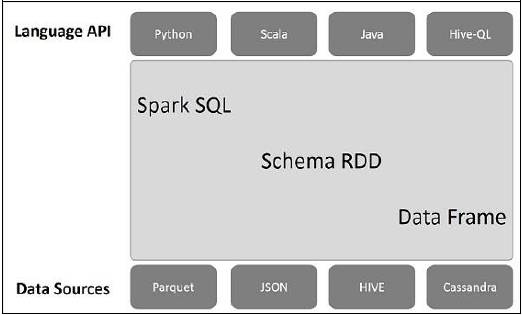
\includegraphics{spark_sql_architecture.jpg}

\subsection{Spark SQL Optimizations(Catalyst)}
Spark SQL operations on DataFrames are represented as abstract syntax trees (ASTs) of operations. Operations can be expressed with Scala quasiquotes, which Scala automatically parses into ASTs. These trees can then be optimzed via "tree surgery."

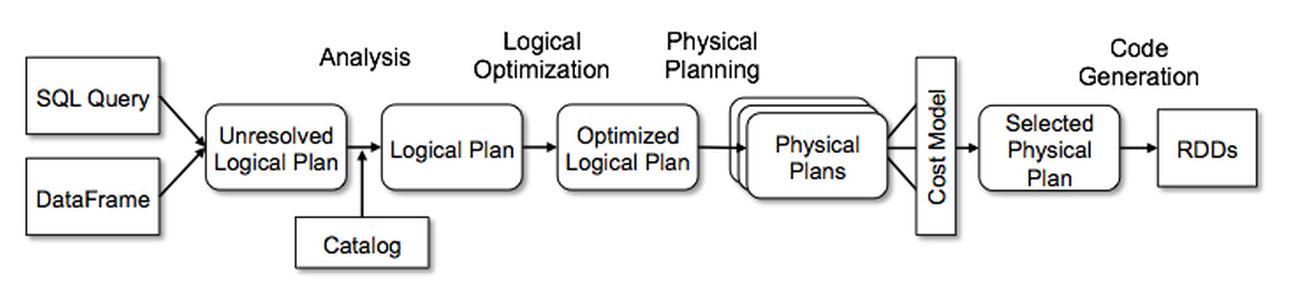
\includegraphics{Screen-Shot-2015-04-12-at-8_41_26-AM.png}

\subsubsection{Constant Folding}
Constant Folding combines multiple operations into one operation. For example, if we the following two add operations, constant folding would combine them into one add operation.

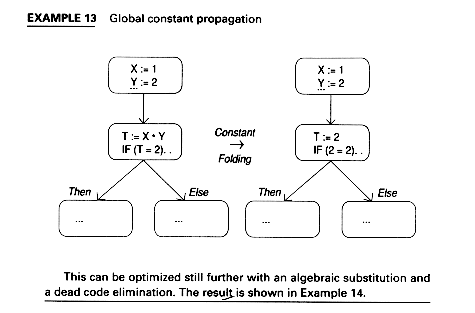
\includegraphics{pg203x13.png}

\subsubsection{Pattern Matching}
Given a recursive definition of a tree, Scala pattern matching is used to replace certain subtrees with new subtrees. The optimizer iterates over the tree, applying predefined pattern matching optimization rules until the tree reaches a "fixed point" and stops changing.

\subsubsection{Predicate Pushdown}
This query optimization takes predicate statements (e.g. "WHERE" clauses) and pushes them closer to the data source, so that less irrelevant data is retrieved as part of the SQL query. 

\subsubsection{Projection Pruning}
This query optimization moves the attributes selected closer to the data source, again to avoid retrieving unecessary data that won't actually be used. 

\subsection{Quasiquotes}
Quasiquotes are a neat notation that lets you manipulate Scala syntax trees with ease:

scala$>$ val tree = q"i am { a quasiquote }"

tree: universe.Tree = i.am(a.quasiquote)

Every time you wrap a snippet of code into q"..." quotation it would become a tree that represents given snippet.

\end{document}

